\section{Durchführung}
\label{sec:Durchführung}

Zur Verfügung stehen ein Ultraschallechoskop, ein Rechner und drei Ultraschallsonden mit den Frequenzen $1 \si{\mega\hertz}$, $2 \si{\mega\hertz}$ und $4 \si{\mega\hertz}$.
Bidestiliertes Wasser wird als Kontaktmittel verwendet. 

Zunächst soll ein Acrylblock, welche mehrere Bohrungen (s. Abbildung (2)) besitzt, mit dem A-Scan untersucht werden. Dazu werden die Abmessungen des Blocks bestimmt.
Mit Hilfe des Impuls-Echo-Verfahrens sollen die Bohrungen lokalisiert werden, indem Wasser auf die zu untersuchende Seite des Blocks getröpfelt wird, und mit der $1 \si{\mega\hertz}$ Sonde der Block untersucht wird.
Mit dem Programm AScan können auf dem Rechner die Schalllaufzeiten an den Stellen der Bohrungen bestimmt werden, woraus die Tiefe der Fehlstellen ermittelt wird.
Der Block wird um $180°$ gedreht und das gleiche wird nocheinmal durchgeführt.

Als nächstes wird das Auflösungsvermögen der benachbarten Fehlstellen 1 und 2 untersucht. Mit dem A-Scan sollen diese beiden Stellen abgetastet werden, wobei alle drei Sonden benutzt werden sollen.

Dann wird der Acrylblock mit dem B-Scan untersucht. Diesmal wird die $2 \si{\mega\hertz}$ Sonde verwendet. Die Sonde muss langsam und mit konstanter Geschwindigkeit über den Block geführt werden, damit ein gutes Bild erzeugt werden kann.
Auch hier wird der Block wieder gedreht, und das gleiche erneut durchgeführt. Aus den erstellten Bildern werden die Abmessungen der Störstellen bestimmt.

Zuletzt soll ein Herzmodell mit dem TM-Scan untersucht werden. Das Herzmodell beseht aus einem Doppelgefäß mit einer beweglichen Membran, die mit einem Gummiball bewegt werden kann.
Das Modell wird zu einem Drittel mit Wasser befüllt und die Sonde wird gerade auf die Wasseroberfläche gesetzt. Mit Hilfe des A-Scans werden die Laufzeiten des Echos bestimmt.
Dann wird das Herzvolumen vergrößert, indem die Membran periodisch gewölbt wird.
Diese erstellte Frequenz wird mit dem TM-Scan aufgenommen, und kann dadurch bestimmt werden. Außerdem wird aus der Kurve das Herzvolumen ermittelt.
\begin{figure}[H]
  \centering
  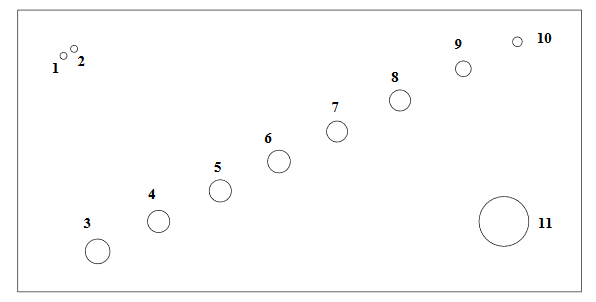
\includegraphics[height=6cm]{acryl.png}
  \caption{Darstellung des Acrylblocks mitsamt Bohrungen. \cite[S.4]{kent}}
\end{figure}